
\section{Basic parallel algorithms \& patterns}

As you might have guessed, parallel programming is a whole field of computer 
science. In the academic world, algorithms are thoroughly analyzed, and scientists come up with new patterns and ideas. I will not give extensive 
comments on the theoretical notions on the algorithm, proof of its complexity, etc... 
The goal is, as you've guessed to give the idea of the main patterns and algorithms and its potential 
applications. As well as intuition of ideas, of how to potentially improve those algorithms.

\subsection{Reduce}
Consider the situation, when we need to add all the array's elements together. In \verb|C++|, one could use 
the STL algorithm \verb|accumulate()| function. In a more primitive implementation, we would do a single for-loop 
and accumulate the results in one variable. The complexity of such an algorithm would then be about $O(n)$, where 
$n$ - the length of the array. However, one could add some parallelism to this algorithm. 
Indeed, at first iteration, what we would 
do is add the 0th element with the 1st, the 2nd with the 3rd, the 4th with the 5th, etc... Notice that 
all of these $\nicefrac{N}{2}$ additions can be done in parallel (that is, each thread does one addition). The next \textit{iteration} would be 
summing the result of the sum of 0th and 1st with the sum of 2nd and 3rd, thus giving a total of 
$\nicefrac{N}{4}$ additions (instead of $\nicefrac{N}{2}$ ) . 
Therefore, the number of necessary divisions in the next step will be half of those, during the previous ones.
As those divisions are performed in parallel, this algorithm looks like a log-scale complexity. 


\begin{figure}
   \centering
   \begin{subfigure}[t]{0.45\textwidth}
        \centering
        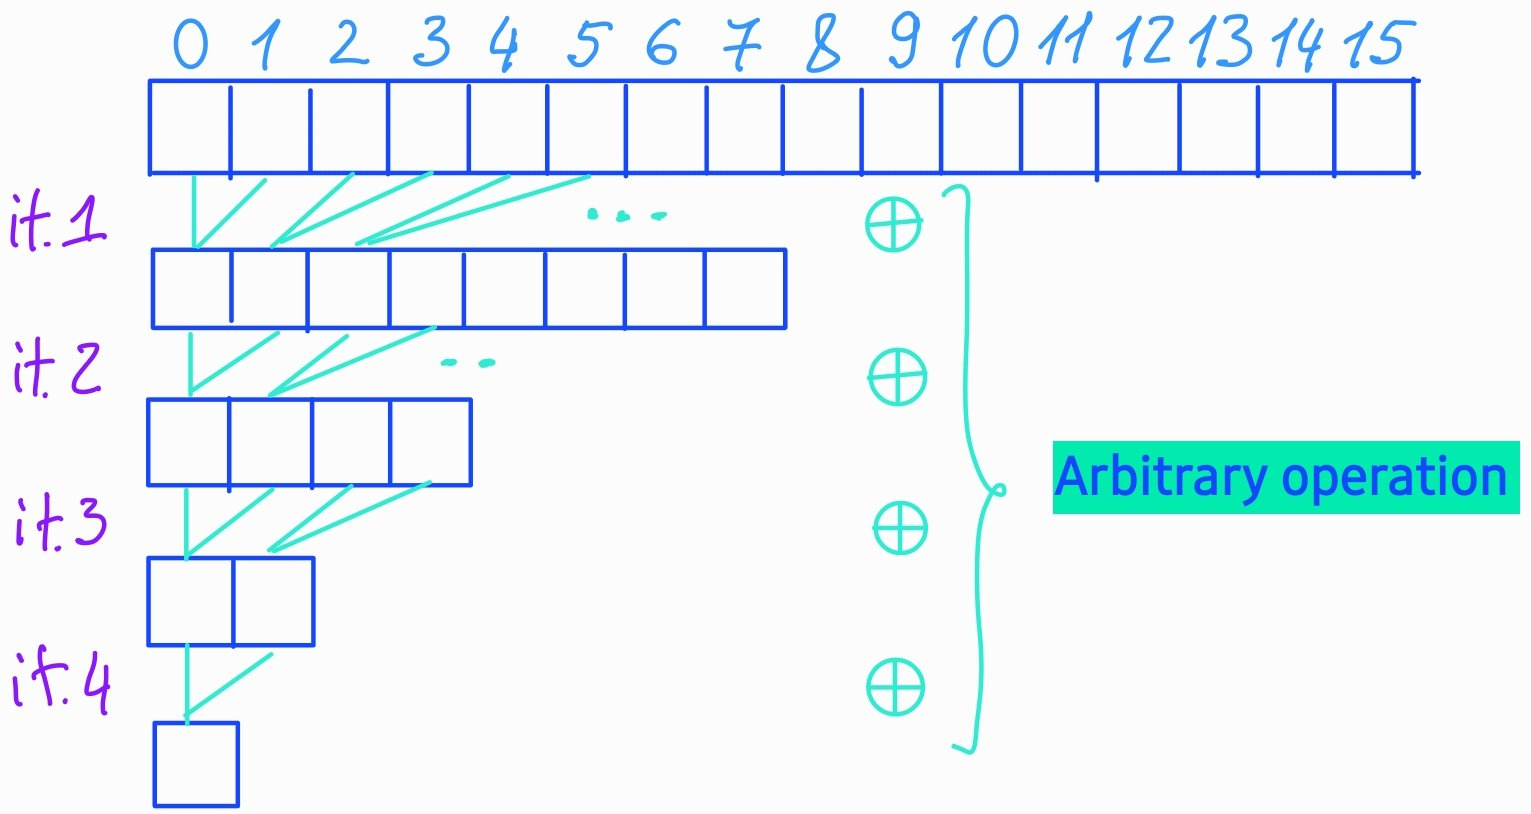
\includegraphics[width=6cm]{pngs/reduce_global.jpg}
        \label{fig:static}
    \end{subfigure}
    \begin{subfigure}[t]{0.45\textwidth}
        \centering
        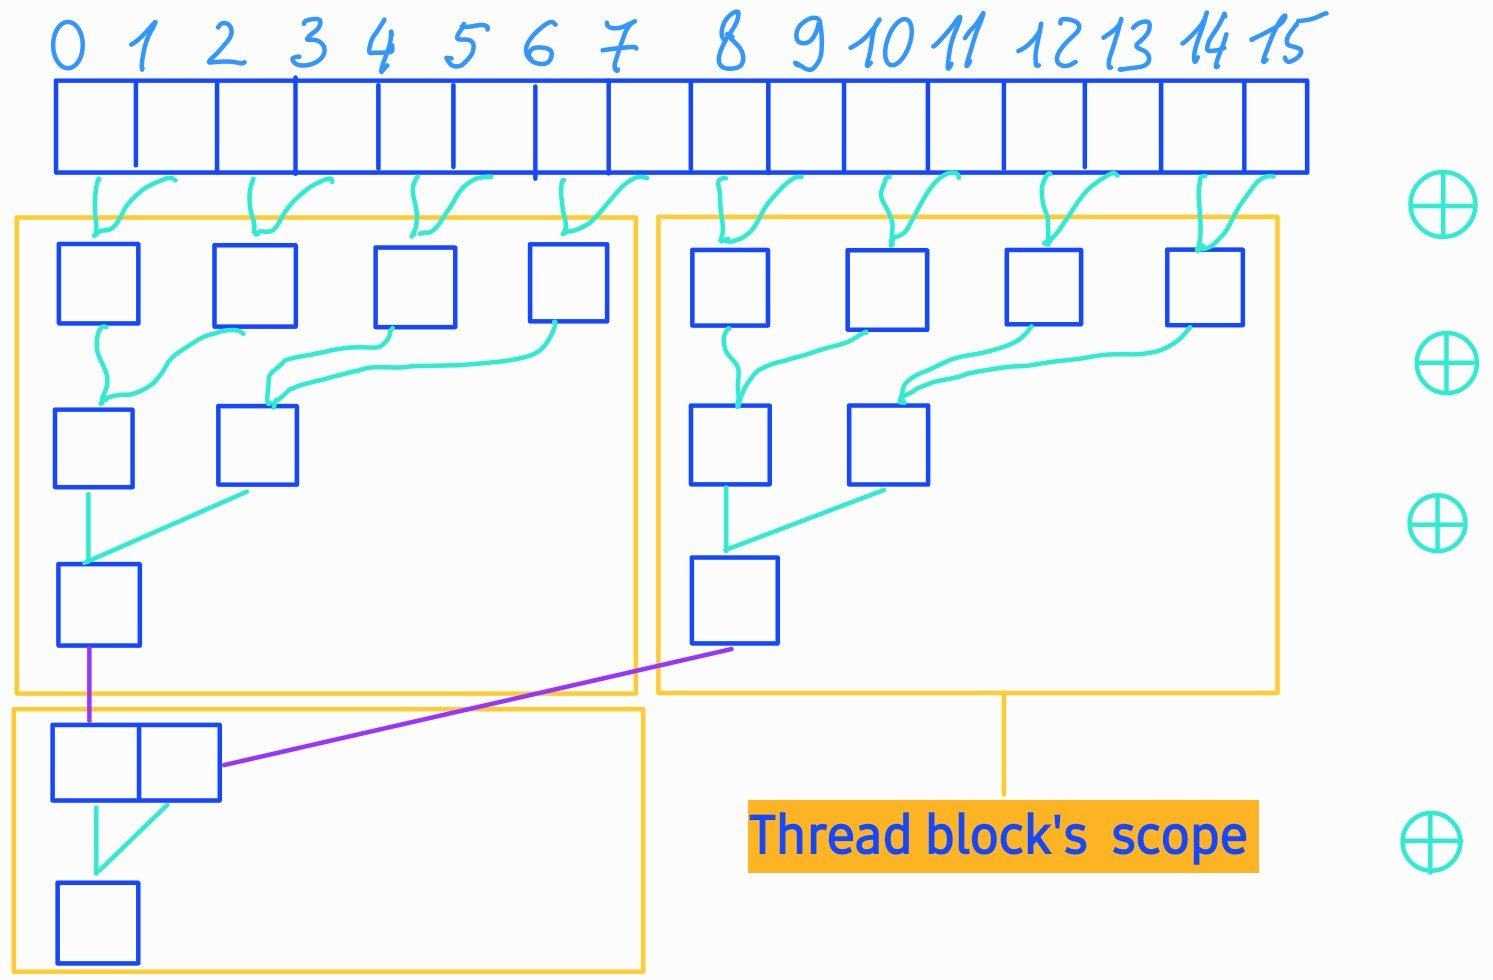
\includegraphics[width=6cm]{pngs/reduce_shared.jpg}
        \label{fig:dynamic}
    \end{subfigure}
\label{fig:reduce}
    \caption{Reduce algorithm with differnet strategies.}
\end{figure}

\subsubsection*{Global memory reduce}
Let's first have a look at a \sout{not-so-}naive implementation of the discussed reduce algorithm on the GPU.
Once again, we're looking at a simplified version of the code, without implementing memory allocation, copy, etc... 
(note that in this case, we use simple global memory with \verb|cudaMalloc()|). The implementation of this is given by \autoref{listing:global_reduction}.


\begin{listing}
\begin{minted}[frame=single, framesep=1mm]{cuda}
__global__ void reduce_global_kernel(float *data_out,\
               float *data_in, int stride, int size) {
int idx_x = blockIdx.x * blockDim.x + threadIdx.x;
if(idx_x + stride < size){
data_out[idx_x] += data_in[idx_x + stride];
}
}

void reduce_global(float *d_out, float *d_in, int n_threads, int size) {
int n_blocks = (size + n_threads - 1) / n_threads;
for (int stride = 1; stride < size; stride *= 2){
   reduce_global_kernel<<<n_blocks, n_threads>>>(d_out, d_in, stride, size);
}
}

//main()
\end{minted}
    \caption{Global memory reduction. \cite{tuomanen2018hands}}
    \label{listing:global_reduction}
\end{listing}

\begin{wrapfigure}{R}{0.45\textwidth}
   \vspace{-0.9cm}
   \begin{center}
   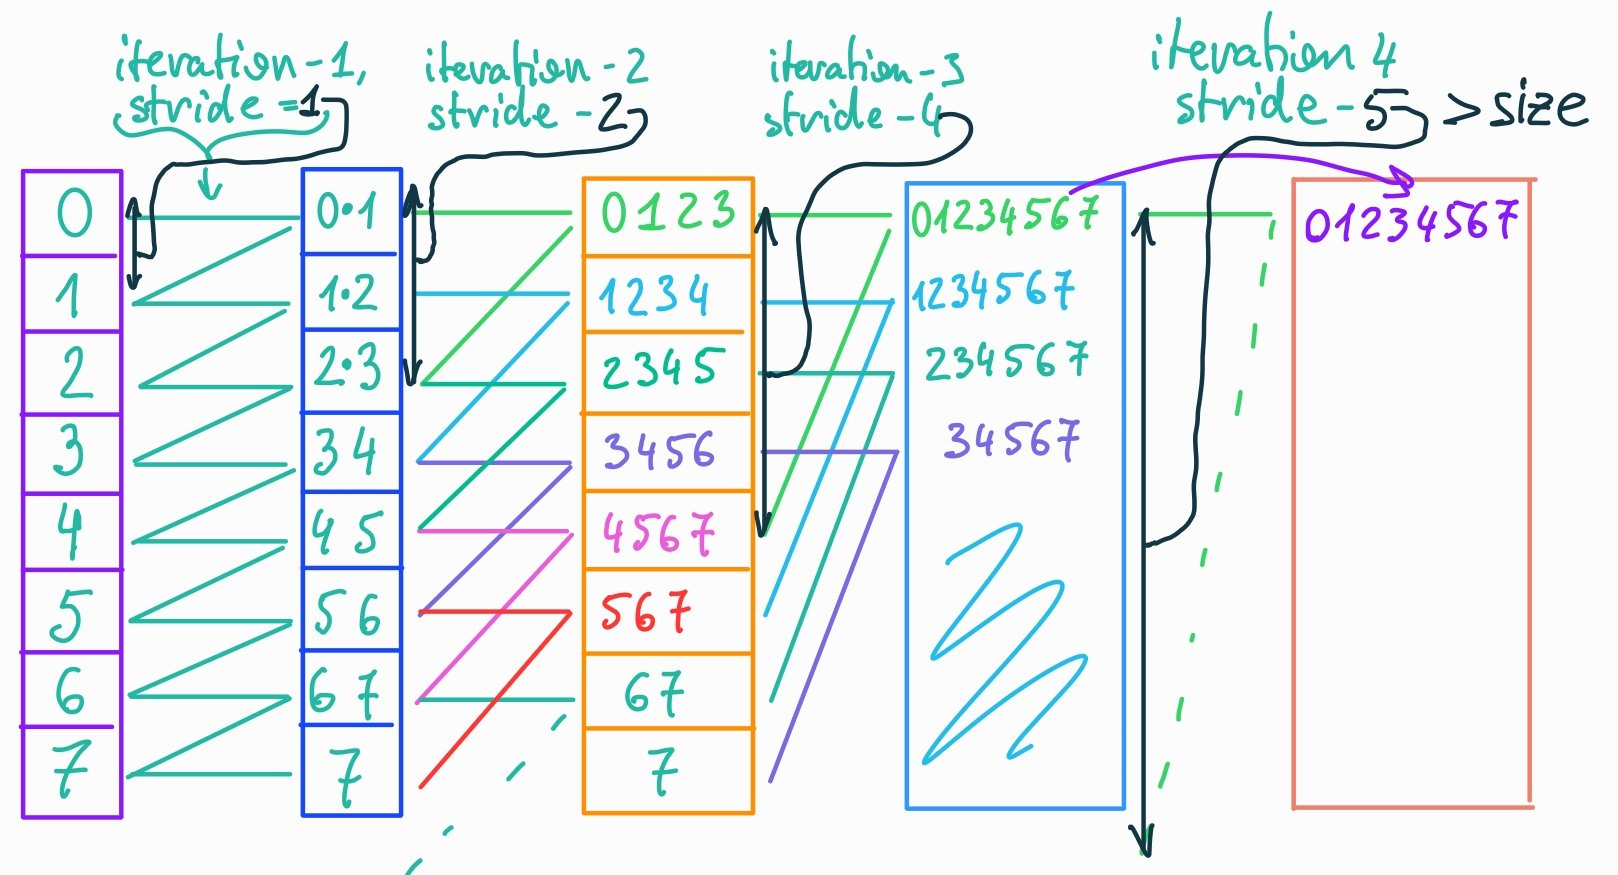
\includegraphics[width=0.45\textwidth]{pngs/reduce_only_global.jpg}
   \end{center}
   \vspace{-0.5cm}
   \captionsetup{justification=raggedleft}
   \caption{The description of every iteration, for the global memory 
   reuction kernel. Note the how stride is doubling every iteration, 
   ,and how the elements are accumulating in the very first (0th) element of the output data. 
   One should understand, that the code works for arbitrary number of blocks, as we're working with global 
   memory, visible to all threads in all blocks}
   \label{fig:reduced_global_only}
\end{wrapfigure}

Okay, let's discuss the \autoref{listing:global_reduction}. First, in the host function, we define the number of blocks. 
In this case, this number is not so important. It would be important to optimize the execution, 
by taking into account the notion of warps, etc... The important part is the loop in the host code and 
the device kernel. We will try to do the debugger's job and inspect the steps. 
During the first iteration, the value of \verb|stride| is 1. The important point is that the thread id, 
computed in the kernel does not depend on the value of the stride. This is because we're working with the global 
memory, and the access is global.

Suppose the size is $32$, partitioned into 1 block. Then for the first iteration, we'll get, 
\verb|out[0] = [0]+[1]|, \verb|out[1] = [1]+[2]|, ... \verb|out[30] = [30] + [31]|. This is exactly the first iteration, 
shown in \autoref{fig:reduced_global_only} (the case of size=8). Then, during the next iteration, we're 
\textit{jumping} over 2 next elements and adding them, in order to get the sum of $N_{stride}$ elements, and save them 
into the \verb|data_out[0]|. Let me mention, that this process is illustrated in the image above \autoref{fig:reduced_global_only}.

This algorithm is, maybe, not easy to understand, but is very fundamental parallel algorithm. Both the algorithm and the 
way of analyzing the problem. However, it can be optimized using the block's shared memory.


\begin{wrapfigure}{R}{0.5\textwidth}
   \vspace{-0.9cm}
   \begin{center}
   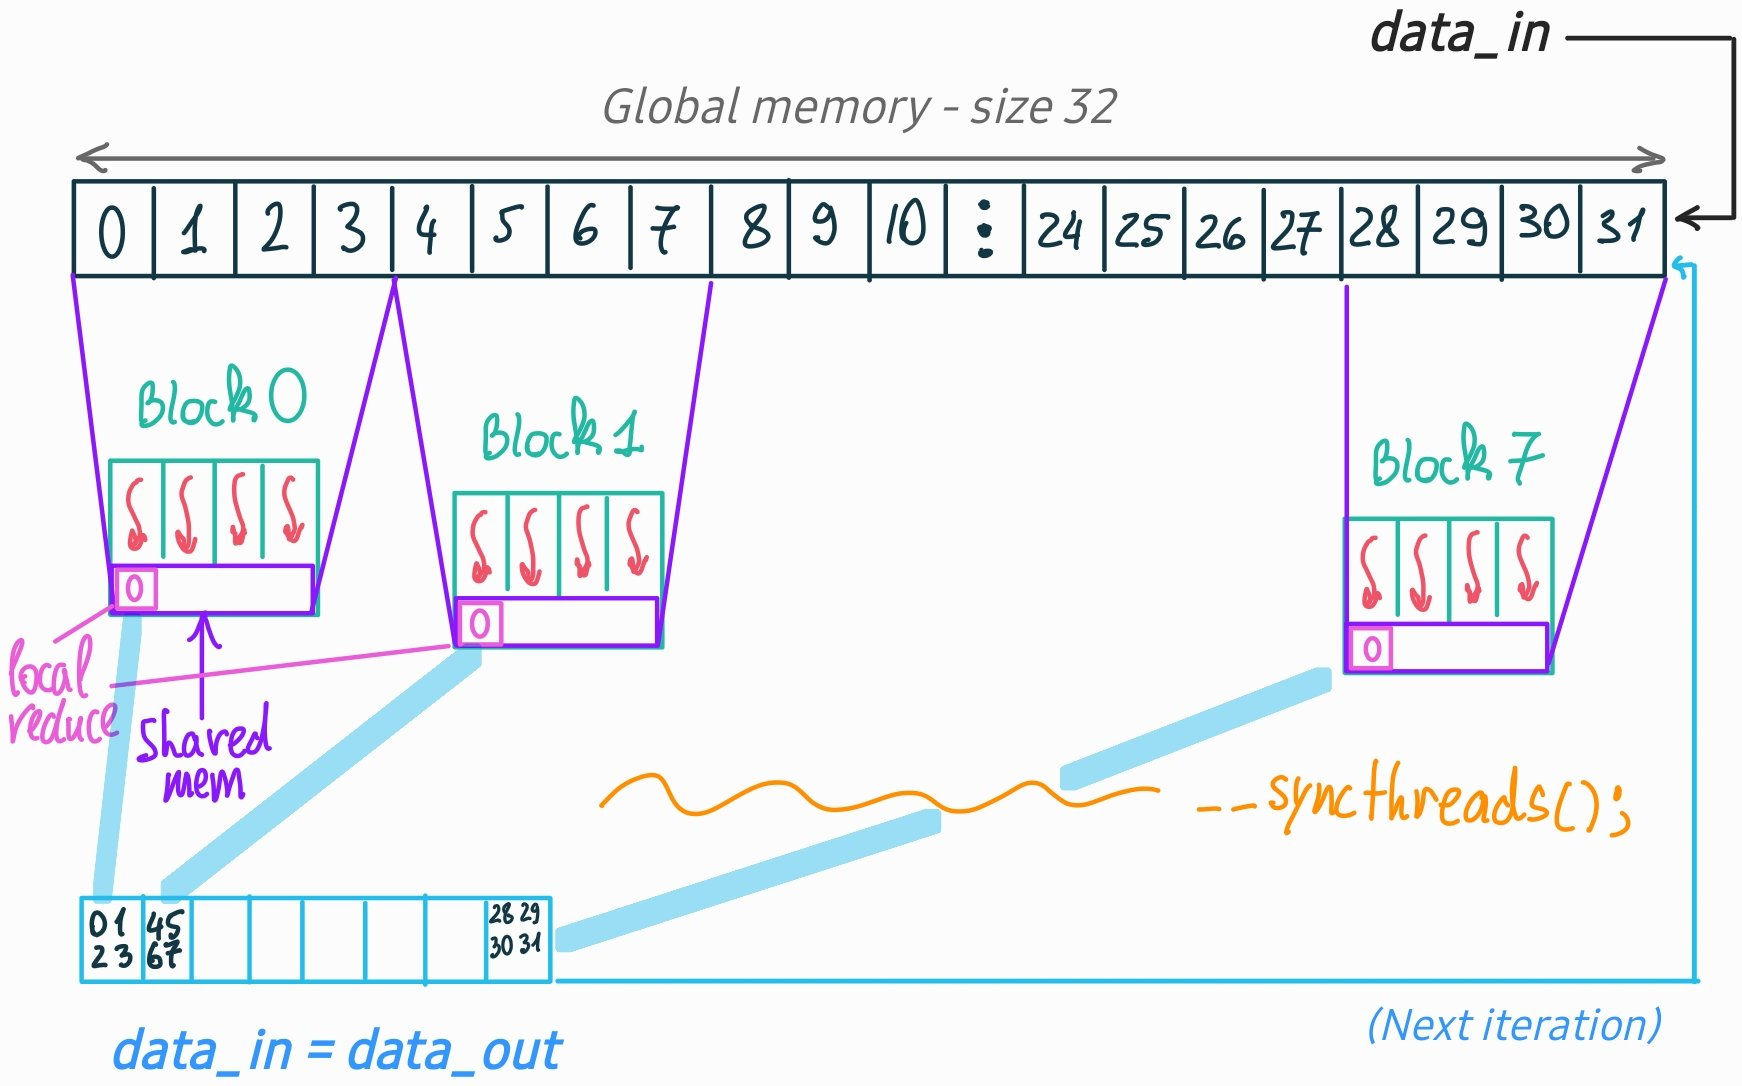
\includegraphics[width=0.5\textwidth]{pngs/shared_reduce.jpg}
   \end{center}
   \vspace{-0.5cm}
   \captionsetup{justification=raggedleft}
   \caption{Reduce algorithm using shared memory.}
   \label{fig:shared_reduce}
\end{wrapfigure}



\subsubsection*{Shared memory reduce}
\label{subsub:shared_reduce}
As we've discussed several times above, shared memory access has low latency. The idea is thus 
to do a local copy of the data to each block. As the shared memory's size is limited, we \textbf{map} the 
data pieces to each block (see figure).

Now, let's try to understand it together in more detail, using well-defined numbers of threads and blocks, 
to make things more illustrative. Trying to keep in mind both the illustration (\autoref{fig:shared_reduce}).

\begin{listing}[ht!]
\inputminted[frame=single, framesep=1mm, linenos=true]{cuda}{cucodes/shared_rreduced.cu}
\caption{Optimized reduce, with shared memory. \cite{tuomanen2018hands}}
\end{listing}

We omit the \verb|main()| function and the host/device memory allocation/copy.
Line $2$ declares the function, which will be calling the kernel. Line $3$ copies the memory 
\verb|cudaMemcpyDeviceToDevice|. This is done in order to make sure we're working with the same memory locally allocated on the device.
This is illustrated with the bottom blue arrow. 
\paragraph*{First iteration}
For the first iteration, we're associating the variable \verb|int size| to be the litteral 
number of elements to be reduced. In our case, it is $32$. The next declared variable \verb|int n_bl| is, 
as the name suggests, the size of the block. As we're working with the shared memory, each shared memory 
will be allocated for one specific block, as shown in figure. In our case, we've chosen \textit{nice} 
numbers, so that \verb|n_thr * n_bl = size = 32|, with \verb|n_thr| - the number of threads per each block.
On line $6$, we're finally invoking the kernel with the initial $8\times 4$ dimensions (the first 2 parameters in the angle brackets). 
The 3rd parameter in the angle brackets is the size of shared memory, that will be assigned to each block. 
We see this syntax for the first time. This is how we allocate the \textbf{dynamic shared memory}, which we will 
discuss a bit later, as well as the last parameter $0$ (ignore that too for the moment).
For now, this is just shared memory allocation, outside the kernel itself. So we've allocated 
$n_{threads}\times size_{float}$ - the exact amount of shared memory, that will be accessed by the 4 threads. 

Let's move to the kernel body itself. First, on line $12$, our usual procedure, we're assigning a personal 
ID to each thread. Line $13$ declares shared memory with size of $n_{threads}\times size_{float}$, specified outside, 
at the kernel call. This is the dynamic allocation of shared memory with \verb|extern| keyword 
(as said, we'll discuss it later). On Line $14$, we're copying the data to shared memory. Remember, 
the size of shared memory is the size of threads in the block (line $6$). Thus the operation 
SH\_DATA[LOCAL\_THR\_ID] is performed. Line $6$ operation is illustrated with the violet lines - the
mapping between the global to shared memory ($[0:3]_{global}\mapsto [0:3]_{block=0},\text{ } [4:7]_{global}\mapsto [0:3]_{block=1}, \text{...} $).
After copying, we are making sure that \textbf{all} the threads are done copying with \verb|__syncthreads()|. Without that, some problems can occur 
(e.g.if we're starting reducing in 0'th block \textbf{before} all the threads within this blocks are done copying its data).

On line 17, we're starting to perform reduction. Let's first try to ignore the \verb|if| 
condition on line $20$, in order to better understand, why is it, and should be here. The 
dummy variable \verb|stride| varies from 1 to the size of the block -
$1\to 2\to 4\to 8\to 16 \to ...$ (in our case till $8$).% Thus for each thread in the block, 
For example, for a local thread with local ID = $0$, the sum of SH\_MEM[0], SH\_MEM[1], SH\_MEM[2] will be accumulated 
within the loop. For thread with local ID = $1$, the sum of SH\_MEM[1], SH\_MEM[2], SH\_MEM[3] will be accumulated. For
thread with local ID = $2$, the sum of SH\_MEM[2], SH\_MEM[3], SH\_MEM[4], will be accumulated, and so on. 
We have now several problems, e.g. the access to SH\_MEM[4], which is out of bounds, as the size of it is the 
save as number of threads ($4$ in our case). 

Consider now the loop on the global scale/scope, as on line $20$, 
we're checking the global thread ID. Then which threads will access the line $21$, for the dummy variable \verb|stride| = $1$? 
These are threads with global ID $0,2,4,6,8,10,12,14,16, ... $, which corresponds to local threads
$\{0,2\}_{block=0},\text{ }\{0,2\}_{block=1}, ...$ (see violet lines \autoref{fig:shared_reduce}). 
On next iteration of the dummy variable \verb|stride| = $2$, only threads with global 
ID's $0,4,8,12,16$ will access the line $21$, which corresponds to local threads $\{0\}_{block=0},\text{ }\{0\}_{block=1}, ...$

Now, taking into account the two aspects, we can say, that for the first iteration of the dummy variable \verb|stride|=1, the 
the threads with local ID's $0,2$, will accumulate SH\_MEM[0], SH\_MEM[1] \underline{into} 
SH\_MEM[0] and SH\_MEM[2], SH\_MEM[3] \underline{into} SH\_MEM[2] respectively. 
For the next iteration of the dummy variable \verb|stride|=$2$, only the thread with local ID's $0$ 
will accumulate SH\_MEM[0] and SH\_MEM[2] into SH\_MEM[0]. \textbf{But remember: } in the previous iteration, 
the sum of SH\_MEM[0], SH\_MEM[1] was stored in SH\_MEM[0] \textbf{and} SH\_MEM[2], SH\_MEM[3] into SH\_MEM[2]. 
Thus, during the last iteration, we've performed the reducing operation within the block and accumulated the sum into SH\_MEM[0]. 
The line $25$ will simply write the value of SH\_MEM[0] to the output, global memory.  The kernel is done. 

\paragraph*{Next iterations} operate the same way as the first. The only thing that is changing is the number 
of blocks, that the GPU will operate with. This does neither change the workflow, nor even the size of 
shared memory within each block. 

It is quite hard \sout{even maybe very hard} to understand the pipeline of the method execution. 
We should re-read the text above again and again, and try to associate it with the \autoref{fig:shared_reduce}.
To recap the reduce process with shared memory:  

 \begin{itemize}
   \setlength\itemsep{-0.5em}
    \item Define the initial number of threads and blocks, such that they cover the whole 
    array to be reduced (note that \#threads - number of elements on which the reduction will be performed locally).
    \item At every iteration, launch the kernel with the \#blocks and update the new size of the array, which 
    contains the previously reduced elements. 
    \item In the kernel : \begin{enumerate}
                           \setlength\itemsep{-0.2em}
                        \item Assign global thread id
                        \item Copy data to the shared memory, from the global memory.
                        \item Perform the reduction in the shared memory locally. With the if condition, make sure that 
                        \begin{enumerate}
                           \setlength\itemsep{-0.2em}
                           \item The memory access does not overflow
                           \item The elements are not added more than once (only add 2 consecutive elements)
                        \end{enumerate}
                        \item Copy the data at 0'th location (the location of the elements accumulated within the block) to the global memory.
                        (in \autoref{fig:shared_reduce}, this corresponds to the blue grid below)
                        
                        \end{enumerate} 
   \item Repeat the kernel, by adjusting the size of the global array, (accessed by kernel at the beginning), 
   controlled by the \# of blocks. 
   \item End when the \#blocks has reached $1$ - when we're left with 1 block, on which we must 
   perform the reduction and store at the 0'th element.
\end{itemize}

Okay, let's now discuss various performance aspects:
\paragraph*{Memory.}Clearly the main difference between the two implementations is 
the usage of memory. The first implementation uses global memory. Every thread goes to 
the global memory to take data, which, of course, takes time. In the shared memory implementation,
the algorithm spends time to initialize the shared memory, which takes time. However, further on, it has lower latency than 
the global one. In general, the performance of the shared memory implementation is better than the global memory. 
Nevertheless, it is almost always advised to implement benchmarking into the code and/or use some 
debugging/benchmarking tools.
\paragraph*{Warps.} One may analyze the code under the warp's viewpoint. Remember, the threads are scheduled 
on the SM, partitioned into groups of 32 - warps. Ideally, they all run in parallel and don't have any 
barriers. Suppose that some threads in the scheduled warp, have some conditions that stops them, so they finish earlier than 
those, who haven't entered the condition. This means that some threads are idle, plus this requires additional, potential 
rescheduling. This problem, which causes throughput inefficiency, is called \textbf{WARP DIVERGENCE}. 
Let's now quickly try to detect warp divergence in both codes. 

In the shared memory implementation, we've got one potential
\verb|if()| condition. Which may cause warp divergence. Indeed, the greater the stride is, 
the more threads will fail the \verb|if(id_x+ stride<size)| condition, thus being idle \& waiting for other threads, who have entered the condition.


The similar issue is in the second code. Indeed, on line  $20$, we have a condition, \verb|if()|. 
The warp divergence is pretty big \footnote{One could potentially deduce the mathematical formulation of warp divergence, 
and evaluate, where is the divergence more present. But for the moment, we will stick with the qualitative approach.}, as 
at every loop, only some threads will \textit{enter} the condition (see the code discussion above), while other will become 
idle. 

To attack these issues, one may use various techniques, potentially discussed in further sections. 
Some of these methods may be very tricky, sometimes requiring built-in CUDA features (unknown for us at the moment), and 
sometime very \textit{primitive} techniques (e.g. \autoref{App.:Primitive operations})

To be fully honest, there is almost never a way to complpetely get rid of warp divergence.
However, it is possible to do small changes to reduce them. 
In this case, we will follow a strategy, that has changed a bit the access of the elements and 
gather/reduce them together. Remember, in the shared memory implementation of reduce, we were 
looking for elements, which are located next to each other. 
We want to modify the memory access of threads, such that the pairs of elements are not necessarily next to each other. To do that, we are dividing the block in 2 parts, and we're adding (reducing) the 
0'th element of the first half and the 0'th element of the second half. We call the dimension
of the half of the block - the stride. Thus we get that SH\_MEM[0] = SH\_MEM[0+stride], 
SH\_MEM[threadId.x] = SH\_MEM[threadId.x+stride]. Note that this expression may cause bad memory 
access, if \verb|threadId.x + stride| is greater than the size of the shared memory. To prevent that, 
we're adding an additional condition - \verb|if(threadId.x<stride)|.
And this process will be done at every iteration
of the for loop in the kernel. Here we are doing nothing but a litteral reduction - \textit{Dividing
the block in half, adding(or any arbitrary operation) the one-to-one elements. When done, 
"throw" away the right block and perform the same reduce on the newly created block.}
From the warp divergence perspective, one may notice that there is still a condition, that will potentially
lead to warp divergence. However, looking at this condition, we can make a statement 
about \textbf{when} will this divergence occur. As the stride vary from \verb|blockDim.x| to 
$0$ being every time divided by 2 (e.g. $64, 32, 16, 8, 4, 2, 1, 0$). The \verb|if| condition will be
omitted \textbf{if and only if} the warp size is less than the stride. Thus, at iterations, when
the stride > $size_{warp}$ no warp divergence will occur, as \textbf{all the threads will pass the condition and there won't be idle threads}. As the warp size is $32$, one can choose the most optimal block dimensions.
Supposedly, the bigger the bloc dimension is, the less iterations will cause warp divergence, the better it is. 

Personally speaking, this code/approach is much easier to understand and visualize than the previous ones, and in addition
a bit faster. However, I wanted to roughly take some course/book's paths, where the reduction is 
presented in this specific order.


\subsection{Scan}

Scan is an another fundamental algorithm in parallel programming. In fact, it is somehow more fundamental than reduce, as the latter is a special case of scan. 
While the reduce algorithm produces a single value from an input array (in fact, the algorithm can operate on any types, as long as it supports a binary operation), 
the result of a scan algorithm is also an array. For example, suppose we're given an array of integers - $\{ 1, 4, 5, 7\}$ and the the binary operation of $+$. Then 
the resulting output of the scan algorithm, would be $\{ 1, 4, 6, 7\} \xRightarrow{+}  \{1, 5, 11, 18\}$ \cite{reeves_ams_nodate}. From that, one can easily 
infer the functionality of the most general scan algorithm - it accumulates the result of the consecutive application of the binary operator, element by element.
More formaly, following the theoretical notions provided in \cite{reeves_ams_nodate}, one defines the inclusive and exclusive scans respectively: 
\begin{align}
  \{x_0, x_1,..., x_n\} \xrightarrow{inclusive scan} \{x_0, x_0 \otimes x_1, ..., \bigotimes^{n}_{i}x_i \}\\
  \{x_0, x_1,..., x_n\} \xrightarrow{exclusive scan} \{\mathds{1}, x_0 \otimes x_1, ..., \bigotimes^{n-1}_{i}x_i \}
\end{align}
, where $\mathds{1}$ is the identity element for the set and the provided binary operation. In the case of addition, $\mathds{1}_{\otimes} = 0$. 

It is clear that the scan algorithm is more complex to implement in parallel. Luckily, there are 2 most popular 
parallel scan algorithms, that are studied in parallel computing classes : Hillis and Steele's algorithm and Blelloch's algorithm \cite{noauthor_prefix_2022}. 
Note that it is very easy to run into very complex descriptions of these algorithms, as well as their alternatives. This is a complex yet promising field 
involving various branches of mathematics and theoretical computer science.
The schematic of the Hillis and Steele's algorithm looks as follows: 

\begin{figure}[ht!]
  \centering
  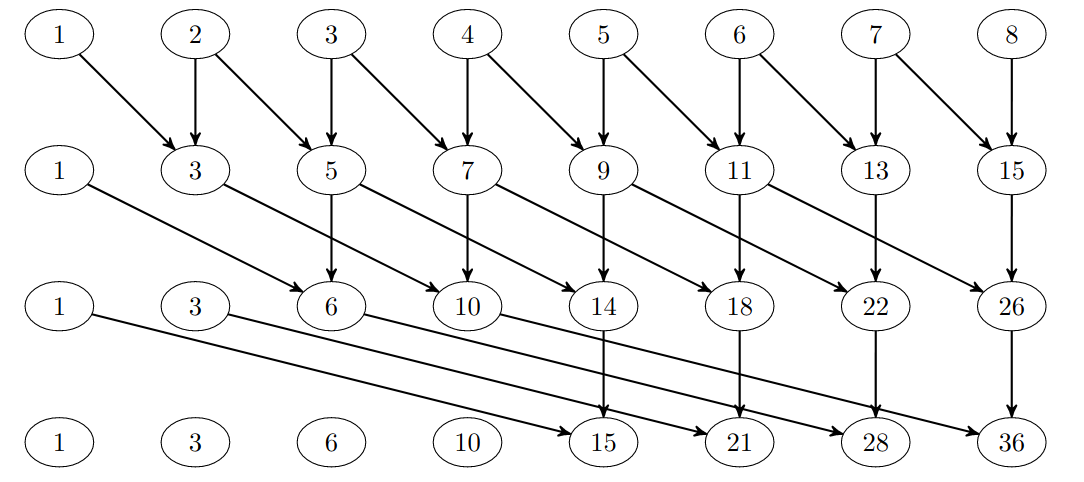
\includegraphics[width=0.8\textwidth]{pngs/hillis_steele.png}
  \caption{The illustration of the (inclusive) scan algorithm. Source from \cite{reeves_ams_nodate}.}
  \label{fig:hillis_steele}
\end{figure}

Okay, let's now try to implement the naive version of the algorithm. In fact, I found very few documents, where this topic is 
approached thoroughly, and where this naive algorithm is further improved. 
So I'll try to describe the idea of the process of how I'd sketch such an algorithm, namely, this naive algorithm.
As usual, the idea is to first design the algorithm, without any consideration about the optimization or whatsoever. 


The main observation of the algorithm depicted on \autoref{fig:hillis_steele}:
\begin{itemize}
   \setlength\itemsep{-0.5em}
  \item If the length of the input array is $N$, then the number of parallel summing operations is equal to $\log_2 N$.
  \item During each parallel operation, we're adding two threads, which are located at a distance we'll call \textsl{offset}.
  \item The \textsl{offset} evolves as $1 \xrightarrow{} 2 \xrightarrow{} 4 \xrightarrow{} 8 ...$.
  \item The final value of the offset seems to be the half of the initial array input.
\end{itemize}

The first assumption that we'll make is that the array will be a power of 2, for example $64$, or $1024$.
The second one, without loss of generality and for simplicity's sake, we'll suppose that the array fits 
into a block. So let's write the operations 
of the pipeline for each iteration: 
\begin{enumerate}
   \setlength\itemsep{-0.5em}
  \item $(in[0] \otimes in[1])\xrightarrow{} out[1]$; $(in[1] \otimes in[2]) \xrightarrow{} out[2]$; $(in[2] \otimes in[3] \xrightarrow{} out[3]) $; $(in[3] \otimes in[4]) \xrightarrow{} out[4]$; etc ...
    \textbf{in $\xleftarrow{}$ out } (performs array copy, i.e. the output array becomes the input array).
  \item $(in[0] \otimes in[2]) \xrightarrow{} out[2]$; $(in[1] \otimes in[3]) \xrightarrow{} out[3]$;
    $(in[2] \otimes in[4]) \xrightarrow{} out[4]$; etc... \textbf{in $\xleftarrow{}$ out }.
  \item $(in[0] \otimes in[4]) \xrightarrow{} out[4]$; $(in[1] \otimes in[5]) \xrightarrow{} out[5]$; etc ... \textbf{in $\xleftarrow{}$ out }.
\end{enumerate}

\begin{listing}
\begin{minted}[linenos=true, frame=single, framesep=1mm]{cuda}
__global__ void naive_scan(int* input, int* output, int size){
  int id = threadIdx.x;
  for(int i = 1; i<=size/2; i*=2){
    if(id < (size)-i){
      output[i+id] = input[id]+input[id+i];
    }
    __syncthreads();
    swap_ptr(input, output);
    __syncthreads();
  }
}
\end{minted}
\label{listing:hillis_steele}
\caption{Hillis-Steele's most naive implementation using global memory. Note that this implementation 
supposes certain condition, such that size of the input array must be inferior to $1024$, and it musts be a power of $2$. 
The first condition is easily modified, as we're anyways working inside the global memory, and the second one is neither a problem, 
as one can always increase the array by adding neutral elements. In the case of addition, the neutral element would be 0.}
\end{listing}

Let's discuss the most basic naive Hillis-Steele's algorithm. This algorithm implementation 
has many problems, and perhaps even slower than the sequential one. 
This implementation uses the global memory (thus increasing latency), has 2 \verb|__syncthreads()| 
calls \footnote{Which is conceptually not a problem, but the need to synchronize threads 2 seems a lot for a 10 line kernel.}. 
%In 
%addition, one may clearly see bank conflicts, when, for example, doing the first iteration of line 5. Indeed, for the first iteration 
%in the $0$'th thread, we're accessing \verb|input[0]| and \verb|input[1]|. At the same time, in thread with index $1$, we're accessing 
%\verb|input[1]| and \verb|input[2]|. This is thus a simultaneous access to one 
Thus we may want to improve this simple scan algorithm by adding shared memory. 
Furthermore, Mark Harris points out that the algorithm performs 
$O(N\log_2N)$ additions, whereas the sequential version of it only does $O(N)$ additions \cite{harris_parallel_2007}. Of course, this 
number-of-additions complexity in parallel algorithms does not impact it as much as in the sequential one 
\footnote{What i mean here, that the number of operations in sequential vs parallel algorithms does not necessarily have a bad impact 
on the algorithm. Indeed, when we are adding 2 vectors, the number-of-additions complexity is the same both for the sequential implementation (simple looping) 
and the parallel implementation. We've however seen that the parallel version of adding vectors is much faster for large vectors. What I want to say 
is that one must dive deeper into theoretical computer science and mathematics, in order to formally analyze the algorithms.}.

Thus, the first improvement is to replace the global memory by the shared one. However, this does not solve the constraint 
of the input vector to be less than the number of threads in the block, as the shared memory's scope is one single block. 
Keeping that constraint in mind, it is quite straightforward to implement the shared memory version of the Hillis Steele's 
algorithm. 


One may try to improve this algorithm further by adding the just-mentioned shared memory \underline{and} removing the constraint of the input array size.
However, I will move on by introducing the next scan algorithm, which is the one that is the most widely used. The Blelloch algorithm is a fundamental 
algorithm, which is taught in all parallel computing courses. The algorithm is indeed not easy to understand, but we will try... The Blelloch algorithm 
performs an exclusive scan (which is different from the inclusive scan, performed by the Hillis-Steele). The algorithm is divided into two main steps. 
The first thing is to construct the so-called \textbf{tree-sum} \footnote{The notion of the tree-sum is not a fundamental notion. However, I've seen this notion in at least two 
sources. So let's call it like that.}

\begin{figure}
  \centering
  \begin{subfigure}[t]{0.45\textwidth}
    \centering
    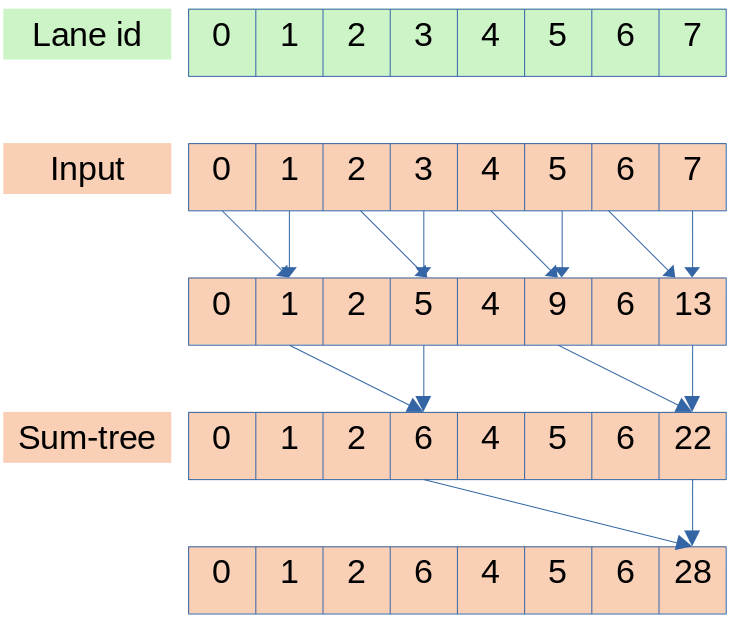
\includegraphics[width=0.95\textwidth]{pngs/blelloch_sum_tree.png.png}
  \end{subfigure}
  \begin{subfigure}[t]{0.45\textwidth}
    \centering
    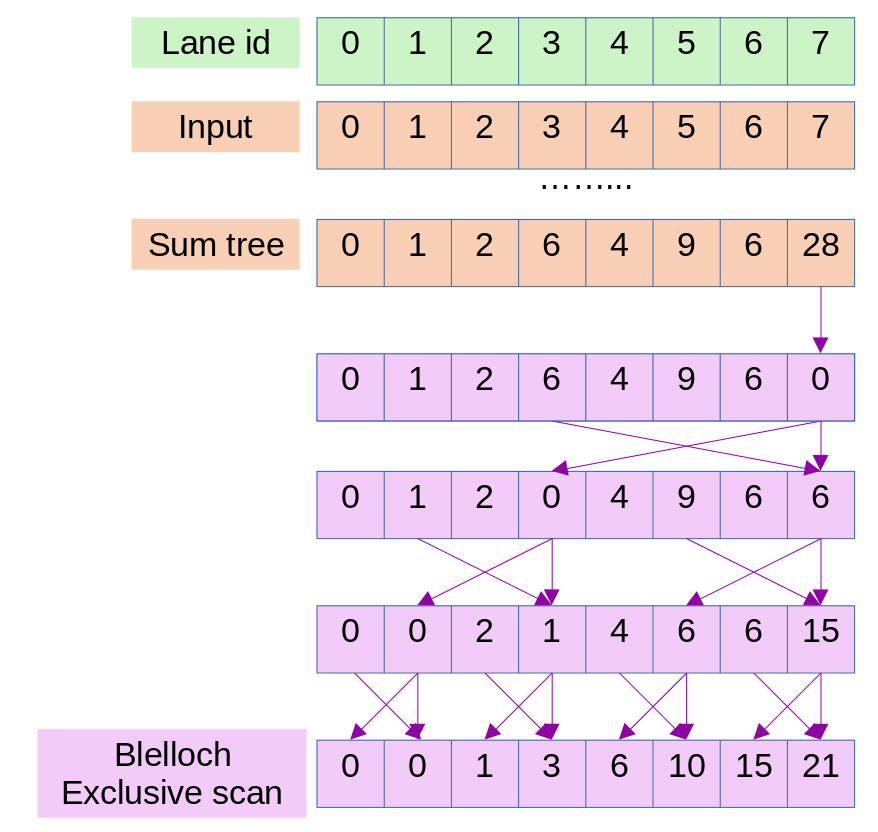
\includegraphics[width=0.95\textwidth]{pngs/blelloch.png}
\end{subfigure}
  \caption{The illustration of the blelloch sum-tree - the first step to the Blelloch scan algorithm (on the left).
  Based on the sum-tree, we proceed to compute the Blelloch algorithm's second part, to find the scan result.}
\label{fig:blelloch_scan}
\end{figure}
The tree-sum is easier to illustrate with a graphical example \autoref{fig:blelloch_scan}. In this simple illustration, 
we have 8 threads, and an input array of size 8, which is simply given by the corresponding lane index.
The in order to get the sum-tree, we first add elements pairwise. Then we add the obtained elements pairwise. 
This process is performed until only one iteration is left. This is where we stop. In other words, this 
can be seen as some kind of reduce operation. Namely, we're just reducing neighbours together. Indeed, 
we're adding $0$ \& $1$, which now becomes the \textit{new first element for the next iteration.} Then, 
we're adding $2$ \& $3$, which now becomes the \textit{new second element for the next iteration.} Once 
this process is done for all elements, we repeat the same thing with the \textit{new first and new second elements just obtained}.
The last element that will be obtained is will be the result of a reduce operation. The difference here between the reduce, is that 
we're keeping those intermediate results, of the reduce operation.
Once this sum-tree is constructed, we now start to compute the Blelloch scan algorithm. This second step of 
the Blelloch algorithm may seem weird, and intuitively, even surprising that it works (at least for me). 
This process of crossing elements down is sometimes reffered to as the \textbf{down-sweep} process. The corresponding 
primitive operation of adding two elements, writing the sum down \textbf{and} reporting the right element to the left \autoref{fig:blelloch_scan} is 
an operation, that has 2 inputs and 2 outputs, which is different from the seen reduce operator, where simply 2 numbers were added and put downwards.
This cross operator is sometimes reffered to as the down-sweep operator. This primitive operator for 2 elements located at $i$ and $j$ 
can be written as something like $in[i] + in[j] \xrightarrow{} out[j]\text{ ; } in[j] \xrightarrow{} out[i]$. 


Let's have a look at the Blelloch scan algorithm, proposed by Mark Harris \cite{harris_parallel_2007} and
\cite{boreskov__nodate}. To be more precise, let's first try to understand the initial step of this algorithm, 
that is, building the mentioned sum-tree:

\begin{listing}[ht!]
\inputminted[frame=single, framesep=1mm, linenos=true]{cuda}{cucodes/blelloch_kernel.cu}
\caption{The algorithm to build the sum-tree.}
\end{listing}

Let's now discuss step-by step, what is happening here. What we do first is allocate shared memory and copy the corresponding 
data to this shared memory. You may have noticed that the number of shared memory is a bit strange. This is however not a 
problem. This is done in all scan algorithm implementations and it is done for convenience. After that, the main loop 
starts the main iteration. The initialization of \verb|d| starts with assigning the value of the half of \verb|n|, which is the size.
After, we check if the thread id is less than \verb|d|. Note that the variable \verb|d| goes from \verb|n/2|, then \verb|n/4|, 
\verb|n/8|, \verb|n/16|, etc... The crucial part is then the computation of \verb|ai| and \verb|bi|, which are the indices of the 2 
variables in the array, that need to be added, when constructing the sum-tree. Once the indices are known, we do the
addition. When this is done, the offset is multiplied by 2. The origin of these 
expression for \verb|ai| \& \verb|bi| can be understood quite well by considering 
separate cases for different \verb|tid|'s. Once again, the idea here is to really go 
over the half of the threads (\verb|d| going from \verb|n/2| to 1, getting divided 
by 2 at every iteration) and adding the elements in the same pattern as described in the 
sum-tree algorithm. The next step is to go over the elements and perform the described 
down-sweep over the array. 



Let's now have a look at the concluding part of the algorithm (\autoref{listing:second_part_blelloch}). We start that by setting the first (here it is the last, as we're 
considering that the algorithm goes from bottom to top) element to the neutral, as we're performing the exclusive scan. Then we 
proceed to do a similar thing as we did during the first sum-tree step. The difference here, is that we're setting the 
\verb|d| to be one, and iterating up to \verb|n|, by multiplying it by 2. The offset now is getting 
decremented, dividing it at every iteration by \verb|2|. Then, similarly, we're checking whether the thread id is less than 
d. Here, the conceptual difference with the tree-sum iteration is that \textsl{we're iterating from the other side of the array.} 
Indeed, at the first iterations (in this second part), very few threads pass the check. Compared to the tree-sum algorithm, where, at the first iterations, many 
threads pass the check. This is why we obtain an \textit{reverse-like} iteration.

\begin{listing}[ht!]
\inputminted[frame=single, framesep=1mm, linenos=true]{cuda}{cucodes/blelloch_end.cu}
\caption{The second, concluding part of the algorithm, performing the blelloch exclusive scan.}
\label{listing:second_part_blelloch}
\end{listing}

At lines $11$ \& $12$, we are computing the indices that are of our interest. You may notice that the 
expression for computing these indices is exactly the same as those in the sum-tree part. As I already 
mentioned, the idea and origin of these expressions seems obvious, once we really consider different 
particular examples of those \footnote{That is, when we fix the number of threads at 8, and consider the iterations for different d's, n's and offsets. \\
Then fix the number of threads at e.g. 16 and consider different values for d's, n's and offsets. And 
etc...}. On lines $15$ and $17$, this down-sweep operator is performed. That is, this cross-operator 
is performed by reporting the i'th element to the j'th, and adding the 2 elements at i.
Finally, we need to syncronize threads before we copy the data. Thus, the final step is to simply copy 
the obtained elements of the exclusive scan to global memory.


The scan algorithm is a fundamental concept in parallel programming. We've seen two \sout{not-so} simple scan algorithms. 
The second implementation comes out to be more efficient than the first inclusive scan. However, it is possible to significantly improve the 
second algorithm too. Indeed, the second algorithm suffers from bank conflicts of multiple orders. I will not comment on these for the moment, 
as these improvements are nicely commented in Harris' Guide on prefix CUDA scan \cite{harris_chapter_nodate}. 

\subsection{Histogram}
An another fundamentally important algorithm is the construction of a histogram, often simply reffered to as histogram.
We can already feel where the multi-threaded architecture can be used. Indeed, a histogram consists of data, that 
we need to partition into different bins. So let's suppose we have $N$ bins, ranging from minimum $m$ to maximum $M$.
Then the idea of an algorithm to do so (in fact, either sequential or parallel) 
will be simple: for some data in the array/dataset $a_0, a_1, ..., a_{n-1}$ of index \verb|i| will be checked whether it is smaller or larger than some value; based 
on that, we will update the count of the corresponding bin by one. The output will therefore also be 
an array of another size (most likely smaller than the input data) of the form $c_0, c_1, ..., c_{k-1}$, where 
the element $\{c_i\}$ holds the number of elements $\{a_k\}_i$ that belong to the bin $\{c_i\}$. We will call it 
either \textit{bin} or \textit{counter}.

For the simplicity, we will consider integer-like bins, that is, the input data $\{a_0, a_1, ..., a_{n-1}\}$, with 
$a_i \in [\![0,255]\!]$, meaning that the number of elements of the output set $c_0, c_1, ..., c_{k-1}$ is of size $256$.

\subsubsection*{Histogram with global memory}
The first and the simplest idea coming to mind is to simply use the global memory. 
That is, the idea is that every thread that was scheduled, will "analyze" one separate element of the 
input data. Then, this specific thread will increment the associated counter of the histogram.
There is however a caveat. All of the threads execute in parallel and there is a possibility 
that at some moment in time, multiple threads would want to increment one same bin of the same 
histogram. In that case, this counter will serve and got change by two (or multiple) different
threads at once. There is thus a data race. This means that we will require atomic operations
(see \autoref{subsub:atomics}) \cite{osnovi_raboti}. 

Let's write the simple histogram kernel, that will make use of global memory and atomic 
operations and comment on it.

So in \autoref{listing:hist_global}, first line, we're initializing the size of the 
input data that we will pass to the kernel. Then, we're calculating the thread ID, that 
the kernel will run on. After, we compute the stride. In this case, the stride only plays the 
role if the number of input data is larger than the number of threads fitting in all the blocks 
in the $x$ direction. Indeed, if it is not the case, the threads will be "indexed further" than the 
available blocks in the $x$ direction, e.g. it can "continue getting indexed further on different SM's". 
This is not very crucial for the scope of the algorithm.
Then, we increment atomically the counter of the histogram using \verb|hist[in[tid]]|. This does work thanks 
to our supposition that the input data ar natural numbers $[\![0,255]\!]$ and the histogram also having 
$255$ bins. Therefore, the inputs also serve as indices.

\begin{listing}[ht!]
\begin{minted}[frame=single, framesep=1mm, linenos=true]{cuda}
#define HIST_SIZE (100*1024*1024)
__global__ void hist_global(int* input, long int size, int* hist_out){
  //compute the thread ID 
  int tid = threadIdx.x + blockIdx.x * blockDim.x;
  int stride = blockDim.x*gridDim.x;
  while(i<size){
    atomicAdd(&(histo[input[tid]]), 1);
    i+=0;
  }
};
\end{minted}
\caption{Global memory, construction of histogram (non-optimal and 
slow implementation of the algorithm.)}
\label{listing:hist_global}
\end{listing}

The problem with this implementation is quite obvious-it's simply 
very slow. Of course, for huge histogram with extremely huge sizes of input, 
there's maybe an small improvement over some sequential CPU version. But in 
a general case, this global memory version of the histogram 
performs slower than the sequential CPU version.



There are two problems with this implementation - one is the usage of the 
atomical operations, which always slows down any program. And the second one is 
the access to the global memory. Thus, when this huge number of threads are trying to 
write into the histogram, the scheduler needs to make sure there is no conflict. This 
slows very much the execution of the program.

To speed up the implementation, we will, as usual, try to implement it using the 
shared memory.

\begin{figure}[ht!]
  \vspace{-0.3cm}
  \centering
  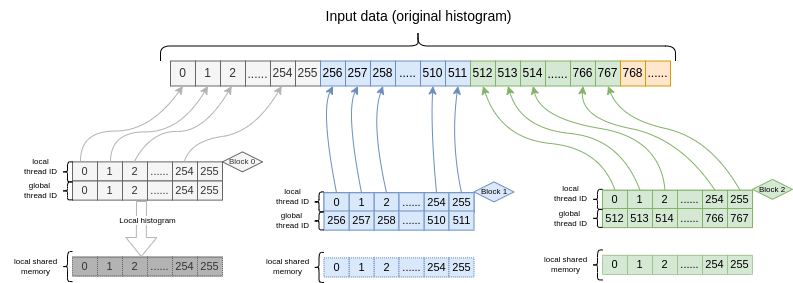
\includegraphics[width=\textwidth]{./pngs/shared_histogram.drawio.png}
  \caption{The working principle of the histogram construction using the shared memory.
  After the computations are done, the results must still be copied further to the global memory. 
  This is not shown on the figure.}
  \label{fig:shared_hist}
\end{figure}

\subsubsection*{Histogram with shared memory}

The idea of the Histogram with using the shared memory is that we're working with the 
histogram locally, by taking a copy of it. In that case, only threads within the block will 
be racing for the histogram, situated in the shared memory. 
In this implementation, we will still use the atomic operations.
However, in this case, the number of threads racing for potentially shared data, will be significantly 
smaller, as well as the time it takes for the threads to access shared memory will also be much smaller 
than in the global memory implementation.

The concept is quite simple and very similar to the previous mechanisms. It is illustrated on \autoref{fig:shared_hist}.

Let's now see how it is implemented in the kernel in question \cite{tehnologija_cuda}. 
We haven't discussed the process of copying the result to the output.
Note that we're copying the data from the shared memory 
from all threads from all blocks simultaneously. 
Therefore, the operation should be atomic (see \autoref{listing:shared_histogram}).

\begin{listing}[ht!]
\begin{minted}[frame=single, framesep=1mm]{cuda}
  __global__ void share_hist(int* in_buf, long int size,
                             int* hist)
{
    //initialize the shared memory
    __shared__ int shared_temp[256];
    //set the just initialized memory to 0
    temp[threadIdx.x] = 0;

    //we synchronize the threads so that we 
    //do not start counting before all was set to 0
    __syncthreads();

    //compute the global thread id
    int tid = threadIdx.x + blockIdx.x*blockDim.x;

    //offset for the case if the entry data 
    //is longer than the number of launched threads
    int offset = blockDim.x*gridDim.x;
    //start counting (note, the while loop executes 
    //more than once in the case if the input data 
    //is longer than the number of launched threads)
    while(tid < size){
      //counting in temp[] if the histogram
      //at position tid should be counted (see fig)
      atomicAdd( &temp[in_buf[i]], 1 );
      i+=offset;
    }

    //syncronize threads, so that operations are done before copying
    __syncthreads();
    //we're now copying the resulting data to the output
    atomicAdd(&(hist[threadIdx.x]), temp[threadIdx.x]);
}
\end{minted}
\caption{Shared memory histogram implementation.}
\label{listing:shared_histogram}
\end{listing}





























